\documentclass[a4paper]{article}

%% Language and font encodings
\usepackage[spanish,es-tabla]{babel}
\usepackage[utf8x]{inputenc}
\usepackage{natbib}
\usepackage{booktabs}
\usepackage{tabu}
\usepackage[T1]{fontenc}
\usepackage{subcaption}
\usepackage{float}
\usepackage{amssymb}
\usepackage{multirow}
\usepackage{comment}

%% Sets page size and margins
\usepackage[a4paper,top=3cm,bottom=2cm,left=3cm,right=3cm,marginparwidth=1.75cm]{geometry}

%% Useful packages
\usepackage{amsmath}
\usepackage{graphicx}
%\usepackage{apacite}
\usepackage[colorinlistoftodos]{todonotes}
\usepackage[colorlinks=true, allcolors=blue]{hyperref}

\renewcommand{\labelenumii}{\theenumii}
\renewcommand{\theenumii}{\theenumi.\arabic{enumii}.}

\title{Detección \textit{in Silico} de Neoantígenos Utilizando \textit{Transformers} y \textit{Transfer Learning} en el Marco de Desarrollo de Vacunas Personalizadas para Tratar el Cáncer }
\author{PhD(c). Vicente Enrique Machaca Arceda}
\date{\today}

\begin{document}
	
	\begin{center}
		\textbf{\Large{UNIVERSIDAD NACIONAL DE SAN AGUSTÍN}} \\
		\textbf{\large{ESCUELA DE POSGRADO} \\
			UNIDAD DE POSGRADO DE LA FACULTAD DE \\
			INGENIERIA DE PRODUCCIÓN Y SERVICIOS}\\
		\vspace*{1.5cm}
		
		
\includegraphics[keepaspectratio,scale=0.6]{img/unsa} \\[.8cm]
		
		
		\textbf{\Large{ Detección \textit{in Silico} de Neoantígenos Utilizando \textit{Transformers} y \textit{Transfer Learning} en el Marco de Desarrollo de Vacunas Personalizadas para Tratar el Cáncer  }} \\
		
		%	Algoritmo de Planificación de Tareas para el \\
		%    Procesamiento de Grandes Cantidades de Datos en  \\ 
		%    Entorno Cluster de Altas Prestaciones}} \\
		
		\vspace*{1.2cm}
		\Large{}
		\begin{flushright}
	Tesis presentada por el Magister: \\
	Vicente Enrique Machaca Arceda \\
	\vskip 0.5cm
	Para optar el Grado de: \\
	Doctor en Ciencia de la Computación \\
	\vskip 0.5cm
	Asesor: \\
	Prof. Dr. Cristian Jose Lopez Del Alamo\\
	%Coorientador: Prof. Dr. Nome do Coorientador
	\end{flushright}
	
	
	\vskip 1cm
	\normalsize{}
	{\bf \large{Arequipa - Perú}} \\
	%\vskip 0.5cm
	{\bf \large{2023}}
\end{center}

	
	
	
	
	
	
	
	
	
	\maketitle
	
	\section{Antecedentes}
	
	El cáncer representa el mayor problema de salud mundial y es la principal causa de muerte, con alrededor de un millón de fallecimientos reportados en 2020. Además, los métodos tradicionales basados en cirugías, radioterapias y quimioterapias tienen baja efectividad \citep{peng2019neoantigen}. En este contexto, surge el desarrollo de la inmunoterapia de cáncer, que tiene como objetivo estimular el sistema inmunológico de un paciente \citep{borden2022cancer}. En esta área, ha emergido la investigación basada en la detección de neoantígenos, hay tres tratamientos: vacunas personalizadas, terapias de células T adoptivas e inhibidores de puntos de control inmunológico. De los métodos mencionados anteriormente, se considera que el desarrollo de vacunas personalizadas  tiene la mayor probabilidad de éxito \citep{borden2022cancer}.\\

Los neoantígenos son péptidos mutados específicos del tumor y se consideran las principales causas de una respuesta inmune \citep{borden2022cancer,chen2021challenges,gopanenko2020main}. El objetivo es entrenar los linfocitos (células T) de un paciente para que reconozcan los neoantígenos y activen el sistema inmunológico \citep{de2020neoantigen,peng2019neoantigen}. El ciclo de vida de un neoantígeno para las células con núcleo se puede resumir de la siguiente manera. Primero, una proteína se degrada en péptidos (posibles neoantígenos) en el citoplasma. A continuación, los péptidos se unen al Complejo Mayor de Histocompatibilidad (MHC), conocido como unión péptido-MHC (pMHC \textit{binding}). Luego, este compuesto sigue una vía hasta llegar a la membrana celular (pMHC \textit{presentation}). Finalmente, el pMHC es reconocido por el \textit{T-cell Receptor} (TCR), lo que desencadena el sistema inmunológico. En este contexto, esta investigación se centra en solucionar el problema de pMHC \textit{presentation} y predecir el enlace pMHC-TCR.\\



	
	

	


		
	
	NetMHCPan4.1 \citep{reynisson2020netmhcpan} es un método 	\textit{pan-specific} considerado como una línea base para la predicción de pMHC-I. Este método utiliza Redes Neuronales Artificiales (ANN). Mejoró sus versiones anteriores al aumentar el conjunto de datos de entrenamiento con 13245212 puntos de datos que cubren 250 moléculas distintas de MHC-I; además, el modelo se actualizó de NN\_align a NN\_alignMA \citep{alvarez2019nnalign_ma}. Además, MHCflurry2.0 \citep{o2020mhcflurry} es otro método de vanguardia; utiliza un predictor de afinidad de unión pan-allelic, un predictor de presentación de antígeno independiente del allele y utiliza datos de Espectrometría de Masas (MS); después de experimentos, MHCflurry2.0 superó a NetMHCpan4.0. En cuanto a la predicción \textit{pan-specific} de pMHC-II, NetMHCIIpan4.0 \citep{reynisson2020netmhcpan} utilizó desconvolución de motif y datos de \textit{eluted ligands} por MS con 4086230 puntos de datos que cubren un total de 116 MHC-II distintos. Por otro lado, NetMHC4.0 \citep{andreatta2016gapped} es \textit{allele-specific}; actualizó sus versiones anteriores, agregando \textit{padding} a los aminoácidos y utilizó ANNs. \\

Los \textit{transformers} se consideran una revolución en la inteligencia artificial y se han aplicado con éxito en varias tareas de procesamiento del lenguaje natural (NLP, por sus siglas en inglés) \citep{patwardhan2023transformers}. Además, estos modelos se han utilizado en la detección de neoantígenos, centrándose en la predicción del enlace pMHC. Por ejemplo, BERTMHC \citep{cheng2021bertmhc} es un método 	\textit{pan-specific} para predecir el enlace pMHC-II; utiliza una arquitectura BERT y transfer learning de \textit{Tasks Assessing Protein Embedding}s (TAPE) \citep{rao2019evaluating}. Los autores aplican una \textit{mean pooling} seguida de una capa \textit{Fully Connected} (FC) después del modelo TAPE. En los experimentos, BERTMHC superó a NetMHCIIpan3.2 y PUFFIN. Además, ImmunoBERT \citep{gasser2021interpreting} también utilizó transfer learning de TAPE; sin embargo, los autores se enfocaron en la predicción de pMHC-I.\\

Además, MHCRoBERTa \citep{wang2022mhcroberta} y HLAB \citep{zhang2022hlab} también utilizaron \textit{transfer learning}. MHCRoBERTa utilizó entrenamiento auto-supervisado a partir de las bases de datos UniProtKB y Swiss-prot; luego, aplicaron \textit{fine-tunning} con datos de IEDB \citep{vita2019immune}. MHCRoBERTa superó a NetMHCpan4.0 y MHCflurry2.0 en SRCC. Por otro lado, HLAB \citep{zhang2022hlab} utilizó \textit{transfer learning} de ProtBert-BFD \citep{elnaggar2021prottrans}; utilizó un modelo BiLSTM en cascada. Además, en el \textit{allele} HLA-A*01:01, HLAB superó ligeramente a los métodos de vanguardia, incluido NetMHCpan4.1, en al menos 0.0230 en AUC y 0.0560 en precisión.\\

Luego, TransPHLA \citep{chu2022transformer} es un método \textit{allele-specific} que aplica \textit{self-attention} a los péptidos. Los autores desarrollaron AOMP, que toma la unión de pMHC como entrada y devuelve péptidos mutantes con mayor afinidad hacia el \textit{allele} MHC. Además, TransPHLA superó a los métodos de vanguardia, incluido NetMHCpan4.1, y es efectivo para cualquier longitud de péptido y MHC, y es más rápido para hacer predicciones. Además, el método DapNet-HLA \textit{allele-specific} \citep{jing2023dapnet} obtuvo resultados interesantes, utilizó un conjunto de datos adicional (Swiss-Prot) para muestras negativas y combinó las ventajas de CNN, SENet (para agrupamiento) y LSTM. La propuesta obtuvo puntuaciones altas; sin embargo, el método no se comparó con métodos de vanguardia.\\


Finalmente, debido a la complejidad del proceso y la gran cantidad de métodos desarrollados, se ha desarrollado software y \textit{pipelines} que pretenden facilitar el uso de estas herramientas. Entre las más recientes tenemos: Somaticseq \citep{fang2015ensemble}, NeoPredPipe \citep{schenck2019neopredpipe}, CloudNeo \citep{bais2017cloudneo}, MuPeXI \citep{bjerregaard2017mupexi}, NeoepitopePred \citep{tran2015immunogenicity}, Neoepiscope \citep{yossef2018enhanced}, pVACtools \citep{hundal2020pvactools}  y NeoFuse \citep{gros2016prospective}. Estas herramientas en su mayoría toman como entrada archivos VCF y archivos de alineamiento Bam, para la detección de mutaciones (inserciones, eliminaciones y fusión de genes) y posibles neo antígenos. 




\section{Problema}

Menos del 5\% de neoantígenos detectados llegan a la membrana y activan el sistema immune \citep{de2020neoantigen, mill2022neoms, bulik2019deep, bassani2015mass, yadav2014predicting}. Además, existen herramientas con buen desempeño en el problema de pMHC \textit{binding}, pero con resultados pobres en  pMHC \textit{presentation} \citep{bulik2019deep}. En este contexto, esta investigación se enfoca en la predicción del enlaces pMHC. Este problema se puede representar como un problema de clasificación binaria, tomando un péptido y el MHC como entrada. Estos son secuencias de aminoácidos, el péptido se pueden representar como: $p = \{ A, ... , Q \}$ y el MHC como: $q = \{ A, N, ... ,Q, E, G \}$. Luego, tenemos que  predecir si $p$ y $q$ pueden enlazarse. %Posteriormente, debemos predecir el enlace pMHC-TCR, el complejo pMHC se puede representar como la concatenación de $p$ y $q$, mientras que que para el caso del TCR, se considera solo la elice $\alpha$ de su proteína, que viene a ser representada como otra secuencia de aminoácidos $r = \{  N, ... ,Q, E \}$. Finalmente, debemos predecir si la concatenación de las secuencias $p$ y $q$ se enlaza con la secuencia $r$.





\section{Justificación}

Los neoantígenos son factores clave en el desarrollo de vacunas contra el cáncer  \citep{borden2022cancer,chen2021challenges,gopanenko2020main}. Si se logra desarrollar un método con un buen desempeño, la inmunoterapia del cáncer basada en el desarrollo de vacunas personalizadas, podría utilizarse como alternativa a otros métodos como radioterapias y quimioterapias. 



	
\section{Objetivos}
	
	\subsection{Objetivo general}
	
	Desarrollar un método basado en \textit{transformers} y \textit{transfer learning} para la detección de neoantígenos en el marco del desarrollo de vacunas personalizadas en la inmunoterapia del Cáncer.
	
	\subsection{Objetivos específicos}
	\begin{enumerate}
		\item Implementar un método basado en \textit{transformers} y \textit{transfer learning} para predecir el enlace péptido-MHC (\textit{pMHC presentation}).	
		\item Evaluar el modelo basado en \textit{Transformers} y \textit{Transfer Learning} para el problema de \textit{pMHC presentation}.
		\item Implementar una herramienta Web para la detección de neoantígenos a partir archivos \textit{Variant Calling File} (VCF).

		

		
	\end{enumerate}

	
\section{Hipótesis}

Un método basado en \textit{transformers} y \textit{transfer learning} puede detectar neoantígenos a partir de la predicción del enlace pMHC.

\section{Variables de investigación}


\subsection{Variable Independiente}

La variable independiente de esta investigación es el modelo basado en \textit{transformers} y \textit{transfer learning}. Este modelo se utilizará tanto para la predicción del enlace pMHC y para pMHC-TCR.

\begin{table}[H]
	\centering
	\setlength{\tabcolsep}{0.5em} % for the horizontal padding
	{\renewcommand{\arraystretch}{1.2}% for the vertical padding
	\begin{tabular}{clp{8cm}}
		\multicolumn{1}{l}{\textbf{Variable}}      & \textbf{Dimensión} & \textbf{Indicador}   \\ \hline                   \\
		\multirow{2}{*}{Transformer} & Base de datos          & Número de muestras \\
		& Hiperparametros          & Arquitectura del modelo, \textit{epochs}, taza de aprendizaje,  \textit{weight decay}  y \textit{early stopping}
	\end{tabular}
}
\end{table}


\subsection{Variable Dependiente}

La variable dependiente, deteminará el desempeño del modelo basado en \textit{transformers}.

\begin{table}[H]
	\centering
	\setlength{\tabcolsep}{0.5em} % for the horizontal padding
	{\renewcommand{\arraystretch}{1.2}% for the vertical padding
	\begin{tabular}{clp{8cm}}
		\multicolumn{1}{l}{\textbf{Variable}}      & \textbf{Dimensión} & \textbf{Indicador}   \\ \hline                   \\
		\multirow{2}{*}{Detección de neoantígenos} & Velocidad          & Tiempo de procesamiento en milisegundos \\
		& Desempeño          & Acierto, \textit{f-score}, \textit{presicion} y \textit{recall}   
	\end{tabular}
}
\end{table}


\section{Metodología de la Investigación} 

En este proyecto, se propone utilizar una arquitectura BERT con \textit{transfer learning}. Analizamos alternativas como TAPE \citep{rao2019evaluating}, ProtBERT-BFD \citep{elnaggar2021prottrans}, ESM-1b \citep{rives2021biological} y ESM2 \citep{lin2023evolutionary} cada una con 92 millones, 420 millones, 650 millones y 15 billones de parámetros respectivamente. TAPE fue entrenado con 30 millones de proteínas, ProtBERT-BFD con 2122 millones de proteínas y 250 millones de proteínas para ESM-1b. Además, ESM-1b obtuvo mejores resultados en precisión de contacto que TAPE y ProtBERT-BFD \citep{rives2021biological}; sin embargo, ya contamos la versión nueva ESM2 \citep{lin2023evolutionary}.\\

Además, HLAB \citep{zhang2022hlab} propuso el uso de ProtBERT-BFD \citep{elnaggar2021prottrans} con un modelo BiLSTM en cascada y superó a NetMHCpan4.1 (método de vanguardia) en el \textit{allele} HLA-A*01:01. Por lo tanto, en este proyecto, proponemos utilizar el modelo preentrenado ESM2 \citep{lin2023evolutionary} con un capa BiLSTM  similar a HLAB \citep{zhang2022hlab}. Para el \textit{fine-tuning}, utilizaremos conjuntos de datos de NetMHCpan4.1 y NetMHCIIpan4.0.\\

En resumen, en la Figura. \ref{fig:proposal}, presentamos la propuesta: primero, se concatenan y se aplica \textit{padding} al péptido y la pseudo secuencia MHC; en segundo lugar, utilizamos el modelo \textit{transformer} ESM2 para obtener una nueva representación de los aminoácidos; finalmente, utilizamos un BiLSTM para predecir el enlace pMHC. 





\begin{figure}[H]
	\centering
	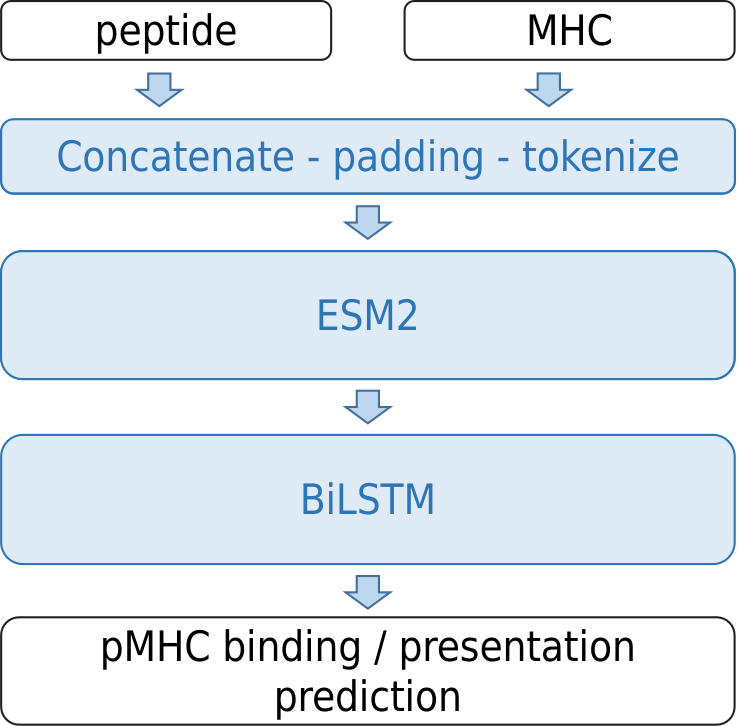
\includegraphics[width=0.35\textwidth]{img/neoantigen/proposal1}
	\caption{Propuesta: Utilizamos el modelo de transformer ESM2 seguido de BiLSTM para predecir el enlace pMHC.}
	\label{fig:proposal}
\end{figure}


\section{Tipo y Diseño de la Investigación}

La investigación es experimental, aplicada y a nivel correlacional. Nos basaremos en experimentos con bases de datos para evaluar el desempeño de método propuesto en la detección de neoantígenos. Además, es a nivel correlacional, porque determinaremos en grado de relación de los parámetros e hiper parámetros del modelo propuesto y su desempeño en \textit{f-score}, \textit{accuracy}, \textit{presicion} y \textit{recall}.



\section{Contenido Tentativo}

\begin{enumerate}
	\item Capítulo I: Introducción
	\begin{enumerate}
		\item Contexto y Motivación
		\item Problema
		\item Objetivos
		\item Hipótesis
		\item Justificación
	\end{enumerate}
	\item Capítulo II: Marco Teórico
	\begin{enumerate}
		\item Inmunoinformática
		\begin{enumerate}
			\item Bioinformática y ADN
			\item Mutaciones
			\item Immunología
			\item Neoantígenos
		\end{enumerate}
		
		\item Deep Learning
		\begin{enumerate}
			\item Machine Learning
			\item CNN, RNN y Transformers
			\item Transfer Learning
		\end{enumerate}		
	\end{enumerate}
	
	\item Capítulo III: Estado del Arte
	\item Capítulo IV: Propuesta
	\begin{enumerate}
		\item Predicción del enlace pMHC
		\item Predicción del enlace pMHC-TCR
		\item Implementación del Pipeline		
	\end{enumerate}
	
	\item Capítulo IV: Resultados
	\item Capítulo V: Conclusiones
	\item Referencias
\end{enumerate}

\section{Cronograma de Trabajo de la Investigación}
En la Tabla \ref{tab:actv}, presentamos el cronograma de actividades por trimestre.

\begin{table}[H]
	\centering
	\setlength{\tabcolsep}{0.5em} % for the horizontal padding
	{\renewcommand{\arraystretch}{1.2}% for the vertical padding
		\caption{Cronograma de actividades por trimestre.}
		\label{tab:actv}
	\begin{tabular}{|p{6cm}|c|c|c|c|c|c|c|c|} \hline
		\textbf{Actividades}                                              & I & II & III & IV & V & VI & VII & VIII \\ \hline
		Revisión sistemática de la literatura                              & x                     & x                      & x                       & x                      &                       &                        &                         &                          \\
		Redacción de un \textit{review} y plan de tesis                             &                       &                        &                         & x                      &                       &                        &                         &                          \\
		Implementación de modelos para la predicción del   enlace pMHC     &                       &                        & x                       & x                      & x                     &                        &                         &                          \\
		Implementación de modelos para la predicción del   enlace pMHC-TCR &                       &                        &                         & x                      & x                     & x                      &                         &                          \\
		Implementación del \textit{pipeline}                                        &                       &                        &                         &                        & x                     & x                      & x                       &                          \\
		Redacción de un paper y la tésis                                   &                       &                        &                         & x                      & x                     & x                      & x                       & x                       \\ \hline
	\end{tabular}
}
\end{table}

\section{Presupuesto de la Propuesta}
En la Tabla \ref{tab:presupuesto}, presentamos el presupuesto para el trabajo de investigación. Este aciende a la suma de 24000 mil soles.

\begin{table}[H]
	\centering
	\setlength{\tabcolsep}{0.5em} % for the horizontal padding
	{\renewcommand{\arraystretch}{1.2}% for the vertical padding
		\caption{Presupuesto. Abreviaciones, PC: \textit{Personal Computer}}
		\label{tab:presupuesto}
	\begin{tabular}{|p{5cm}|c|c|c|} \hline
		\textbf{Insumo o material}    & \textbf{Unidades} & \textbf{Precio} & \textbf{Total} \\ \hline
		PC de escritorio              & 1                 & 5000            & 5000           \\
		PC virtual para entrenamiento & 1                 & 4000            & 4000           \\
		Hosting                       & 1                 & 1000            & 1000           \\
		Inscripción a congresos       & 2                 & 4000            & 4000           \\
		Viaje a congresos             & 2                 & 10000           & 10000          \\ \hline
		\textbf{Total}                         &                   &                 & \textbf{24000}         \\ \hline
	\end{tabular}
}
\end{table}

\clearpage
	
	\bibliographystyle{apalike}
	\bibliography{bibliography}
	
\end{document}